\section{Introduction}
\label{s:intro}

Security problems in cloaking, phishing site, suspicious site, non-compliant
content, malware, dishonest behavior.

Given a form to the user and tell him, you can get some money if you sigh up,
but this form is not delivered to Google.



Cloaking, used by spammers for the purpose of increasing the visiting rates of
their website, as well as to circumvent censorship, has been a challenging
spamming technique to search engines. Recently, there is a rising trend of
employing cloaking in advertisement spam~\cite{li2012knowing}.  The motivation
of cloaking is to hide the true nature of a website by delivering different
semantic content users versus censors.

Spammers use user agent, referer, IP etc based cloaking techniques to
differentiate censors and normal users.

Cloaking is popular due to the low cost to setup and lack of efficient technique
to detect. Spammers use user agent, referer, IP etc based cloaking techniques to
differentiate censors and normal users.

There are two major challenges in cloaking detection (A) revealing the uncloaked
content (B) differentiating cloaking from naturally dynamic changes of the same
page. Existing approaches pretend to be the user, e.g. use proxies, set referer,
to reveal the uncloaked content, but spammers could detect and block them. An
intuitive way is to collect data from user directly. However, it is hard to
collect sufficient data for comparison while protecting user privacy.


\begin{figure}[t]
  \centering
  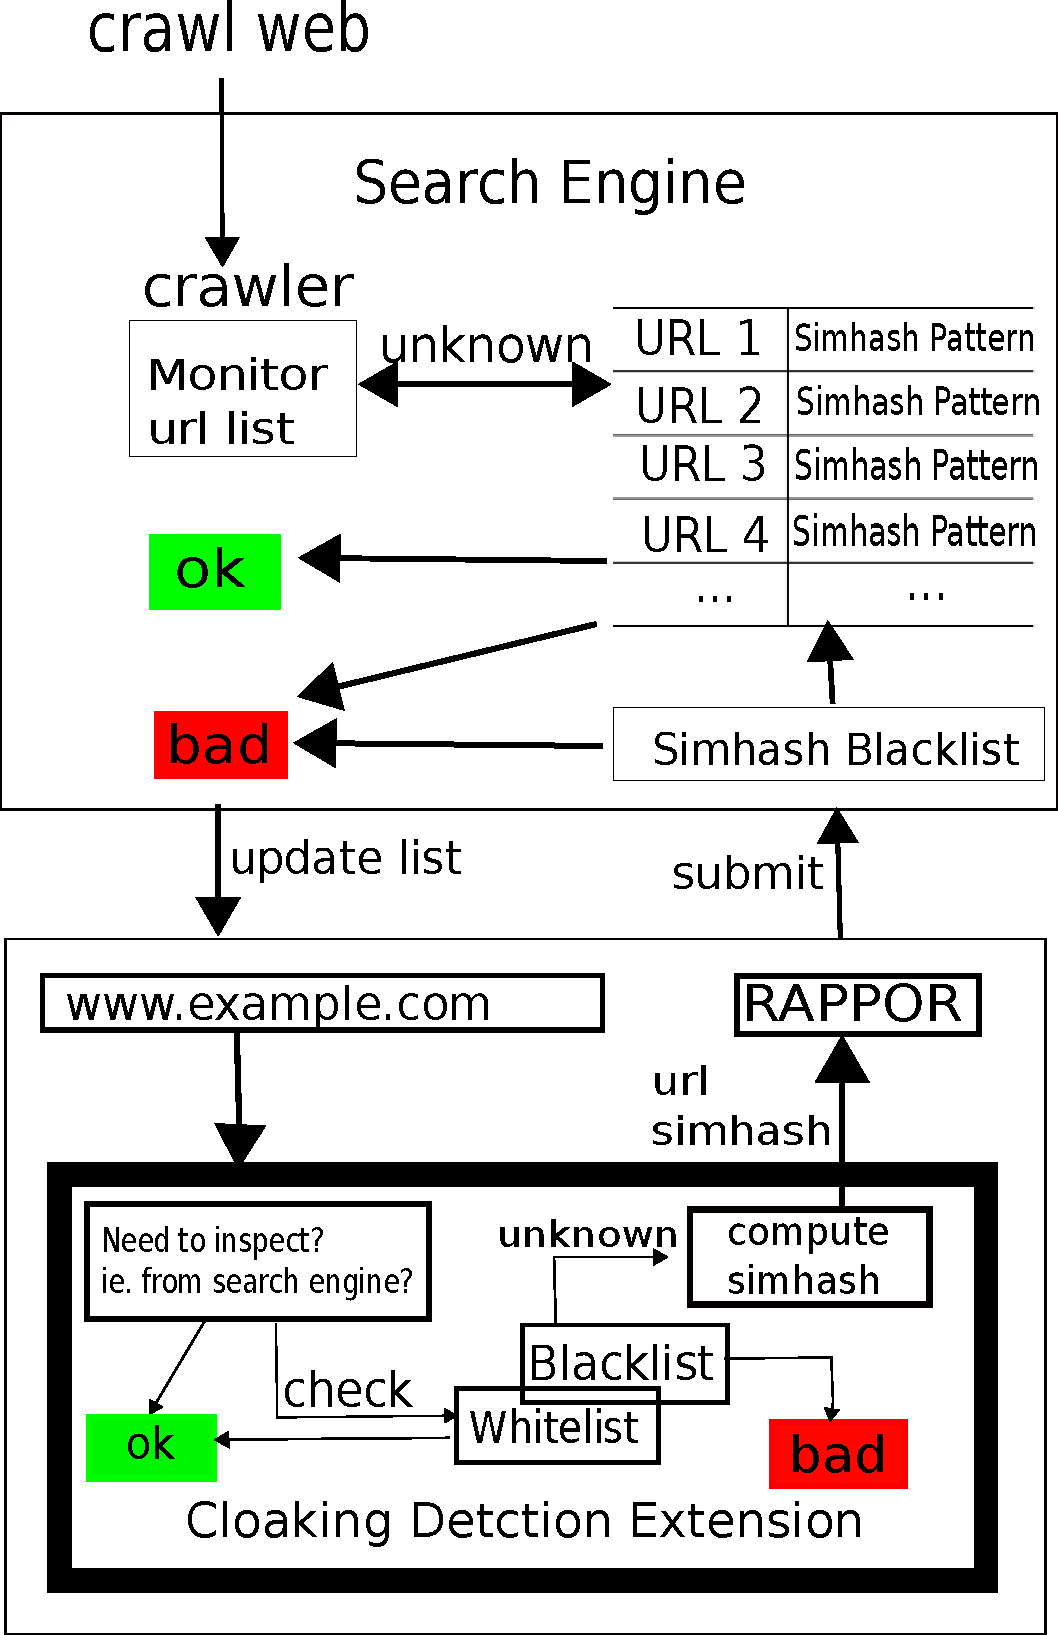
\includegraphics[width=.5\textwidth]{fig/workflow}
  \caption{Workflow of the Proposed cloaking detection sysetem}
  \label{fig:workflow}
\end{figure}




The workflow ~\autoref{fig:workflow} is to collect page contents simhash on the user side, and compare
them to simhash of the same link from ad serving company to find cloaking. When
the differences of the simhashes are significantly large, the page is marked
cloaking. We generate two simhash for page content and structure respectively.
Intuition behind this is, simhash difference between different sites are larger
than different visits of the same site. We build a two-phase system to detect
cloaking: cluster learning phase, and cloaking detection phase. In the cluster
learning phase, an ad company visit urls and generate simhash from its content
with its owned IP, and learn pattern and distribution of the simhashes, i.e.
simhash-based website model. In the cloaking detection phase, the ad company
collects simhash from its users. Compare them with learned patterns, return
cloaking score or mismatch. Results on have shown data set show that we can
achieve more than 95\% True positive rate with 5\% false positive rate for page
content simhash and 100\% true positive rate with 2\% false positive rate for
structure simhash. If we define cloaking as mismatch in both page content
simhash and structure simhash (intersection of mismatches in both case), we can
achieve more than 99\% true positive rate with 1\% false positive rate.


In our detection result, we have observed many cloaking cases, where URL are
completely different, while the content are similar or even the same.
We argue that, the foundamental reason for them to do this is the low cost of
getting a new URL and lack of efficient way to detect spammy content.
Based on this observation, we propose content based blacklist to raise the bar
for reusing spammy content. This approach leverages the most popular use of
simhash - near duplicate detection. For spammy pages, in order to evade our
detection, they not only need to change URL rapidly, but also update their
content everytime, which can be expensive in their current mode if they want
every copy their website to be different and have meaningful and stay attractive
to user.


This paper makes the following contributions:
(1) Introduce simhash-based website model to represent the content and layout
dynamics of a page.
(2) Propose the idea and framework to detect cloaking and protect user through crowdsourcing,
with low traffic overhead and privacy guarantee for user.
(3) Use of simhash-based website model, in cloaking detection, with better FPR
and TPR.
(4) Detect cloaking in both SEO and SEM , showing the seriousness of cloaking
problem in SEO and SEM.
(5) Examine the cloaking strategies employed by attackers.


The remainder of this paper is structured as follows. Section
~\autoref{s:related-work} provides a
technical background on cloaking and simhash, and related work in cloaking
detection. Section ~\autoref{s:swm} introduces the simhash-based website model.
Followed by a description of cloaking detection framework design in 
Section ~\autoref{s:framework}. Section ~\autoref{s:implementation} describes the 
prototype that we implemented and Section ~\autoref{s:experiment} shows our results,
followed in  Section ~\autoref{s:discussion} by a discussion of attack
model and defenses.



More fascinating text. Features\endnote{Remember to use endnotes, not
footnotes!} galore, plethora of promises.\\


According to ~\cite{lin2009detection}, many cloaking software packages support
IP cloaking, and some even provide services to periodically refresh the list of
crawlers’ IP addresses. Therefore, IP cloaking is hard to detect. To the
author's knowledge, there is no known work that can solve IP
cloaking.


